\documentclass{article}

\usepackage{textcomp}
\usepackage{amsmath}    % need for subequations
\usepackage{graphicx}   % need for figures
\usepackage{verbatim}   % useful for program listings
\usepackage{color}      % use if color is used in text
\usepackage{subfigure}  % use for side-by-side figures
\usepackage{hyperref}   % use for hypertext links, including those to external documents and URLs
\usepackage{cite}
\usepackage{float}
\usepackage{natbib}
\usepackage[utf8]{inputenc}
\usepackage{simplemargins}
\usepackage{setspace}
\usepackage{multirow}
\usepackage{url}

\usepackage{etoolbox}
\usepackage{lipsum}

\setallmargins{1in}
\onehalfspacing

\linespread{1.8} % line space

\patchcmd{\thebibliography}{\section*}{\section*}{}{}

% don't need the following. simply use defaults
%\setlength{\baselineskip}{15.0pt}    % 16 pt usual spacing between lines
%\setlength{\parskip}{3pt plus 2pt}
%\setlength{\parindent}{20pt}
%\setlength{\oddsidemargin}{0.5cm}
%\setlength{\evensidemargin}{0.5cm}
%\setlength{\marginparsep}{0.75cm}
%\setlength{\marginparwidth}{2.5cm}
%\setlength{\marginparpush}{1.0cm}
%\setlength{\textwidth}{150mm}

\usepackage{xcolor}
\hypersetup{
    colorlinks,
    linkcolor={red!50!black},
    citecolor={blue!50!black},
    urlcolor={blue!80!black}
}





\title{Seismic Hazard Estimation of Northern Iran Using Smoothed Historical Seismicity}
%\author{



%\begin{center}
%\linespread{1}\Large\bfseries {Naeem Khoshnevis}$^*$\\  Graduate Research Assistant \\  University of Memphis \\ Center for Earthquake Research and Information \\   nkhshnvs@memphis.edu\\   3890 Central Ave. Memphis TN 38152 \\ Phone (901) 678-2007 \\    \\ \textbf{Shima Azizzadehroodpish}  \\ Graduate Research Assistant \\ University of Memphis \\ Center for Earthquake Research and Information \\ szzzdhrd@memphis.edu\\  3890 Central Ave. Memphis TN 38152 \\ Phone (901) 678-2007 \\  \\ \textbf{Chris H Cramer}   \\ Research  Associate  Professor \\  University of Memphis \\ Center for Earthquake Research and Information \\ ccramer@memphis.edu \\  3890 Central Avenue, Memphis, TN 38152   \\ Phone (901) 678-4992 \\

%\end{center}

% }

\begin{document}
%\thispagestyle{empty}
\maketitle


\newpage

\begin{center}
\textbf{Naeem Khoshnevis$^*$} \\ Graduate Research Assistant \\  University of Memphis \\ Center for Earthquake Research and Information \\   nkhshnvs@memphis.edu\\   3890 Central Ave. Memphis TN 38152 \\ Phone (901) 678-2007\\
\vspace{10 mm}
 \textbf{Shima Azizzadehroodpish}  \\ Graduate Research Assistant \\ University of Memphis \\ Center for Earthquake Research and Information \\ szzzdhrd@memphis.edu\\  
\vspace{10 mm}
\textbf{Chris H Cramer}   \\ Research  Associate  Professor \\  University of Memphis \\ Center for Earthquake Research and Information \\ ccramer@memphis.edu \\
\vspace{10 mm}
\textbf{Ricardo Taborda}   \\  Assistant  Professor \\  University of Memphis \\ Department of Civil Engineering and \\ Center for Earthquake Research and Information \\ rtbrdros@memphis.edu\\

\end{center}




\newpage


\begin{abstract}
In this study we conduct a new probabilistic seismic hazard assessment for northern Iran, using recently confirmed ground motion prediction equations and updated seismic catalogs. We evaluate seismic hazard over three tectonic seismic zones (Alborz Mountain Range, Azerbaijan and Kopeh-Dagh) using smoothed historical seismicity. In this model, events are not assigned to specific faults and are assumed to be potential seismogenic sources, spatially gridded to cells. We decluster historical and instrumental seismicity to compute the rate of earthquakes in each grid, and smooth these rates to account for uncertainty in the spatial distribution of future earthquakes. We assume each grid cell has spacing of $0.1^{\circ}$ in latitude and $0.1^{\circ}$ in longitude and count the number of earthquakes in each of them. We use Gaussian filter to smooth the fraction of earthquakes in incremental intervals of magnitude. For this article, in order to consider the seismicity rate, we consider all historical and instrumental earthquakes with magnitude above 3. To calculate the seismic hazard we defined two models based on structural damage threshold magnitude, including Mw 4.5 and Mw 5 with weight of 0.3 and 0.7, respectively. Seismicity parameters are calculated for each seismic region, and smoothed seismicity is calculated separately for each.  We add the probability of exceedance of all regions and present the smoothed seismicity hazard in northern Iran. The horizontal peak ground acceleration is selected as the ground motion parameter. The results are assessed in terms of the expected peak ground acceleration (PGA) with a 10\% and 2\% probability of exceedance in 50 years for rock site conditions. The seismic hazard map for northern Iran is presented. The maximum seismic hazard values are 0.44 $g$ and  0.74 $g$ for 10\% and 2\% probability in exceedance in 50 years, which are calculated in both Azerbaijan and Alborz tectonic seismic region. The result of 10\% probability of exceedance in 50 years are in close agreement with current Iranian code of practice for seismic design of building.
\end{abstract}

\smallskip
\noindent \textbf{Keywords: } Seismic hazard - Spatially smoothed seismicity - Northern Iran


\section{Introduction}

Iran is situated over Himalayan-Alpide seismic belt, which has frequently experienced strong shaking induced by earthquakes. The occurrence of these earthquakes has imposed notable destruction to the buildings and lifelines, and unfortunately, has caused extensive loss of human life. These earthquakes are categorized in various tectonic seismic zones. Different tectonic seismic regions have been defined for Iran in different studies.  Fig.~\ref{fig:Iran} shows the study region and different seismotectonic classification. Some of these studies defined more detailed division \citep{Nowroozi1976, Tavakoli1999}, and some of them defined one simplified province \citep{Stocklin1968, Takin1972, Berberian1976}. \citet{Mirzaei1998} divided Iran into five tectonic regions, including Azerbaijan-Alborz, Kopeh-Dagh, Zagros, Central-East Iran, and Makran. Regarding the other tectonic seismic regions, \citet{Karimiparidari2013} divided the Azerbaijan-Alborz tectonic seismic region into two regions, which are Azerbaijan and Alborz Mountain Range (hereinafter, Alborz). Azerbaijan, Alborz and Kopeh-Dagh tectonic seismic regions encompass most of northern Iran. Northern Iran has many highly populated cities (e.g., Tehran, Tabriz, and Mashhad), in which many destructive earthquakes have been reported.\\
\noindent
In northeastern of Iran, at least four historical earthquakes with $M>7$ struck in less than 200 years (1209, 1405) near the city of Neyshabur. Historical records show that in 1209, the district of Neyshabur from Neyshabur city in the west to Daneh village in the east was totally destroyed \citep{Berberian1999}.\\
\noindent
In the north western of Iran, a study of the seismic history of Tabriz based on available data shows that this region has been seismically active since 634 A.D. The historical earthquake data (pre 1900) illustrate that in earlier times the region was destroyed several times by major earthquakes. In 858, Tabriz was completely destroyed by a massive earthquake; the 1040 earthquake caused more than 50,000 causalities, and in 1936 due to the earthquake in Tabriz, most of the buildings fissured and even some collapsed \citep{Berberian1999}. Most recently, earthquakes with $M_w$ 6.1 in 1997 and $M_w$ 6.4 in 2012 occurred in Ardabil and Tabriz, respectively. These earthquakes caused around 1500 casualties and extensive damage \citep{USGS_ardabil,USGS_tabriz}.\\
\noindent
In north central Iran, in the Alborz region, a historical earthquake sequence occurred over a longer time period of 1100 years. At least three damaging historical earthquakes ruptured adjacent segments of the Mosha fault for a continuous distance of nearly 200 km: 958 A.D. (western segments), 1665 A.D. (eastern segments), and 1830 A.D. (central segments) \cite{Berberian1999}. Recently, the 1990 $M_w$ 7.4 Manjil-Rudbar earthquake caused extensive loss of life and significant damage \citep{USGS_manjil}. Based on existing documents, Tehran city and ancient Rey city have been destroyed completely several times by severe earthquakes with magnitudes greater than 7 \citep{Ambraseys2005}. \\
\noindent
Regarding historical earthquakes and the need for constructing new buildings and infrastructure, different seismic hazard analyses were conducted in Iran. Dividing Iran into 20 tectonic seismic regions, \citet{Tavakoli1999} prepared iso-acceleration contour lines and seismic hazard zonation for return periods of 75 and 475 years or 50\% and 10\% probability of exceedance in 50 years, based on major known lines and area source models. According to their study, North Tabriz fault zone and north of Tehran fault zone are in the highest acceleration contour. Maximum mean acceleration in the vicinity of these tectonic elements is predicted to be around 0.45 $g$ and 0.3 $g$ for a return period of 475 and 75 years, respectively. In the smaller scale, using the logic tree approach to compensate for uncertainties in the attenuation relationship, \citet{Ghodrati2003} presented a probabilistic seismic hazard assessment of metropolitan Tehran, the capital of Iran. The results showed that the PGA ranges from 0.27-0.46 $g$ for a return period of 475 years and from 0.33-0.55 $g$ for a return period of 950 years. In the last three decades, different seismic hazard analysis studies substantially improved the Iranian Code of Practice for Seismic Resistant Design of Buildings \citep{BHRC2014}. \citet{Ghodrati2013} conducted a seismic risk assessment for the city of Tehran using the Hazus method \citep{FEMA2003}. They represent that these efforts successfully decrease the total mean damage ratio in Tehran from 0.302739 in 1996 to 0.272859 in 2006.  Even though the results are satisfactory, the continuous improvement of procedures for defining the seismic hazard at regional (national) and local levels is essential for the optimum design of earthquake-resistant structures. In this study we use another model to overcome the aleatory and epistemic uncertainties regarding earthquake location and source mechanism in northern Iran.\\

In this study we used smoothed seismicity \citep{Frankel1995}. We divided northern Iran in three seismotectonic regions including Azerbaijan, Alborz, and Kopek Dagh. We computed seismic parameters and catalog completeness in these regions. Zagros and Central Iran seismotectonic regions have considerable effect on the Northern part. We used \citet{Karimiparidari2013} seismicity parameters in these regions.  We consider the MW5 earthquake as a threshold magnitude  for structural damage. In order to consider damage to the historical masonry building we also considered Mw45 as a threshold for structural damage to this building. 


\begin{figure} [H]
\centering
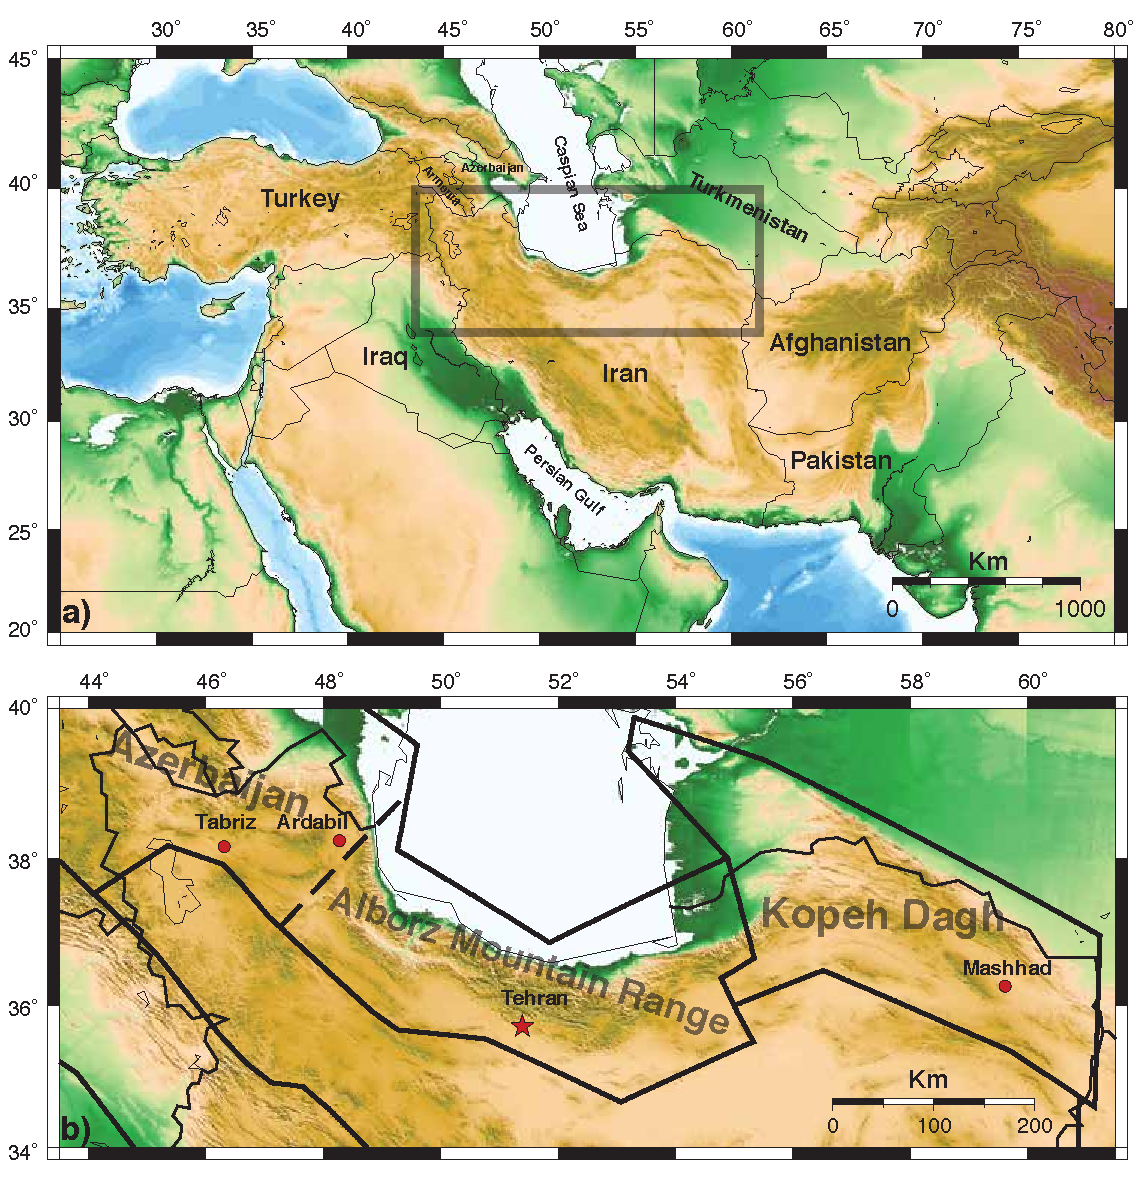
\includegraphics[scale=0.7]{figures/pdf/Figure1.pdf} 
\caption{ a) Map of Iran and surrounding countries. The study area is presented in gray box. b) The study area containing seismotectonic provinces after \citet{Mirzaei1998}, and location of big cities. Dashed line is the subdivision that is proposed by \citet{Karimiparidari2013}. }
 
\label{fig:Iran}
\end{figure}





\noindent
Recently, northern Iran has been studied in detail from different seismological points of view. \citet{Nemati2015} studied the most recent 200 years' seismicity in northern Iran. The frequency of shocks vary widely from one mainshock per 6 years (0.17 event/ year) for the Azerbaijan region to 13 earthquakes per 4 years for the Kopeh-Dagh (3.25 event/year) region. Recorded events and a partially quiet period suggest that strong earthquakes must be expected in Alborz within the next decade, which may cause significant damage to northern Iran. Using newly recorded data, \citet{Zafarani2014} defined the most appropriate attenuation relationship for use in the Azerbaijan, Alborz and Kopeh-Dagh regions. In this study we use an updated catalog from International Institute of Earthquake Engineering and Seismology \citep{IIEES} and the recently confirmed attenuation relationship for northern Iran \citep[i.e.,][]{Kalkan2004} in order to conduct seismic hazard analysis from background seismicity. We follow \citet{Frankel1995} approach to calculate hazard from background seismicity for northern Iran. This differs from the traditional approach in which area source zones are drawn around seismicity or tectonic provinces for the calculation of seismic hazard \citep{Cornell1968}. \\
\noindent
Having limited knowledge in seismic sources, \citet{Frankel1995} used this approach to map seismic hazards in central and eastern United States. The major features of Frankel's approach are to abandon tectonic seismic zones and to use point sources in seismic hazard analysis. This method is simpler for hazards calculation and is based solely on recorded seismicity history. In the smoothed-seismicity approach we avoid choosing zone boundaries that are sometimes poorly delineated by data and drawn by subjectively merging geological and seismological information. Even though probabilistic seismic hazard involving fault sources is more realistic and accurate, recognizing sources could present considerable uncertainty. \citet{Masson2006} studied 19 points of the GPS network that have been installed in the framework of French-Iranian cooperation. At some stations (e.g., the ATTA station) they expect to record significant movement, based on the region's historical activity.  Surprisingly, they recorded velocity of $0\  mm/yr$. \\
\noindent
The smoothed-seismicity method simply assumes that patterns of historical earthquakes predict future activity. Using background seismicity, \citet{Cao1996} conducted a seismic hazard estimation study in southern California. They concluded that one could obtain similar results implementing background seismicity to those obtained by introducing zones for areas with well-recorded seismicity patterns. \citet{Lapajne1997} used spatially smoothed seismicity modeling to acquire a seismic hazard outlook in Slovenia. They defined 4 different models with different correlation distances, including a model based of the total released seismic energy. They gained an acceptable PGA in comparison with other seismic hazard approaches. \citet{Akinci2004} estimate the seismic hazard in central and northern Italy using smoothed historical seismicity. Their results showed that the smoothed seismicity approach gives reasonable regionalized results without introducing seismogenic zones. This approach has also been used in many regions with different seismicity patterns \citep{Wesson1999, Klein2001, Hamdache2008, Kalkan2009, Moschetti2014, Boyd2008}. We generate maps of peak ground acceleration with 2\% and 10\% probabilities in exceedance of 50 years in northern tectonic seismic zones, including Azerbaijan, Alborz, and Kopeh-Dagh and in central-eastern Iran and a small portion of the northern Zagros region. Since we do not introduce faults into the model, our results show variability due only to the characteristics of seismicity and ground motion. 

\section{Seismic regions and seismicity rate}
With respect to different seismicity rates of the regions \cite{Nemati2015}, as well as the completeness of the seismic catalog, the study region is divided into three zones. Each of these zones is characterized by its respective seismicity parameters values, including b-value and maximum magnitude ($M{_{max}}$). A review of Iran's historical earthquakes (pre 1900) is provided by \citet{Ambraseys2005}. \citet{Karimiparidari2013} converted all historical earthquakes to a unified magnitude ($M_w$), which we use as a historical catalog. The International Institute of Earthquake Engineering and Seismology of Iran \citep{IIEES} has reported the instrumental data, which also involves earthquakes from border countries which have considerable affect in the seismicity of Iran's border cities. 
In the present study, historical data are integrated with instrumental data. For the purpose of this research, each seismic region is defined as a rectangular area bounded by latitudes of $34^{\circ}-40^{\circ}$ N, and longitudes of $43.5^{\circ}-48^{\circ}$ E, $48^{\circ}-58^{\circ}$ E, and $58^{\circ}-61.5^{\circ}$ E for Azerbaijan, Alborz, and Kopeh-Dagh, respectively. 

\subsection{Alborz Mountain Range (Alborz)}
Tehran region has active reverse faults, which are parallel to the northwest-trending structural gain of the Alborz Mountains belt. Here a series of historical earthquakes occurred within a time period of more than 1100 years. Four earthquakes with magnitude more than 7 devastated the Tehran region in four centuries period, from 743 to 1177, but in the last 800 years, only one earthquake at 1830 has struck this region. At least three damaging earthquakes in 958 (western segments), 1655 (eastern segments), and 1830 (central segments), ruptured adjacent segments of the Mosha fault, located in northern Tehran \citep{Berberian1999}.
The North Tehran Thrust (NTT) adds more complexity due to the presence of south-dipping reverse faults, which are in part blind, such as the Davudieh, Shian, and Bagh-E Feyz \citep{Berberian1999}.
The northwest continuation of the Alborz Mountains, known as the Rocks of the Talesh Mountains, have been thrust northeastward and eastward over rocks of the south Caspian depression. An earthquake with Ms 6.0 in 1978 led to a focal mechanism consistent with a low-angle thrust \citep{Berberian1999}.



\subsection{Azerbaijan}
There were three earthquakes from 1721-86 that ruptured the North Tabriz Fault system from southeast to northwest. The Tabriz region is in the Araxes structural block of northwestern Iran, southwest of the continuation of the western Alborz Mountains towards the Caucasus. The North Tabriz Fault (NTF) is a complex northwest-trending structure, which contains evidence observed on aerial photographs, and vertical displacement with the north side up, of right-lateral strike-slip displacement \citep{Berberian1999}.
The NTF system and nearby reverse faults ruptured from southeast to northwest in three earthquakes over 65 years: the Shebli earthquake with magnitude 7.3 in 1721 on the southeastern NTF with a surface rupture more than 35 km long, reported by \citet{Jones1834} the Tabriz earthquake with magnitude 7.4 in 1780 on the northwestern NTF, with a surface rupture more than 42 km long and vertical separation of 2 to 4 $m$; and the Marand-Mishu earthquake with magnitude of 6.3 in 1786 on the Mishu reverse fault and the Sufian segment of the NTF. Another earthquake with  magnitude 5.5 struck the Tasuj reverse fault farther west in 1807 and an earthquake of M 6.7 took place along the South Bozqush reverse fault farther southeast in 1879 \citep{Berberian1999}.
Prior to the 1721-86 earthquake sequence, Tabriz was shaken by earthquakes in 858 (M 6.0), 1042 (M 7.3), 1273 (M ~ 6.5), and 1304 (M 6.7). However, their meizoseismal zones are not well known and so could not be used to identify which faults were responsible for them. Earthquakes in 1273 and 1304 were temporal clusters like the 1721-86 events, but the direction of propagation is not known \citep{Berberian1997, Berberian1999}.


\subsection{Kopeh Dagh}
The main Kopeh-Dagh fault system has experienced some historic earthquakes. Ashgabat, the capital city of Turkmenistan, was destroyed by an earthquake of Ms 7.2 in 1948 and destroyed more than 30 villages in Iran. This was the strongest earthquake to strike this region since at least 1455 \citep{Berberian2001}.
The main Kopeh-Dagh fault consists of several partly overlapping segments parallel to the overall $NW - SE$ structure with step-overs. The regions of overlap are characterized by shorter south-dipping thrust faults striking about $E - W$ \citep{Berberian2001}. \citet{Trifonov1978} reported active displacement along the main Kopeh-Dagh fault for more than 500 km. 
Massive destruction of the capital city of Mithradatkert is attributed to the 10 BC event Ms 7.1, roughly 30 kilometers from the border of Iran (Nesa mound) \citep{Berberian2001}.
The Neyshabur sequence of four earthquakes between 1209 and 1405 respected the segment boundary between the Neyshabur and Binalud reverse fault system \citep{Berberian1999}.



\section{Magnitude Conversion}

In this study we use two sets of data, i.e., historical and instrumental seismic catalogs. We use the historical catalog reported by \citep{Karimiparidari2013}, which is converted into $M_w$ magnitude. Fig.~\ref{fig:historical} shows the historical earthquakes (pre-1900) in northern Iran. The instrumental data has been reported mainly by the International Institute of Earthquake Engineering and Seismology of Iran \citep{IIEES}, and are reported in $M_L$ magnitude type. In this study we use the relationship that proposed by \citet{Karimiparidari2013}, to convert local magnitude into moment magnitude. 

\begin{figure} [H]
\centering
\includegraphics[scale=0.8]{figures/pdf/Figure2.pdf} 
\caption{Historical earthquakes of Iran (pre 1900). Different colors represent different year of occurrences and size of circles are proportional to the earthquake magnitude. }
\label{fig:historical}
\end{figure}

\section{Declustering}

It is generally assumed that the seismicity of each tectonic seismic source follows a Poissonian occurrence process. Therefore, in order to accomplish this, we declustered the earthquake catalog. In compiling the catalog of events, foreshocks and aftershocks were removed using a declustering methodology \citep{Gardner1974}. Fig.~\ref{fig:instrumental} shows the epicenter of declustered instrumental  earthquakes.

\begin{figure} [H]
\centering
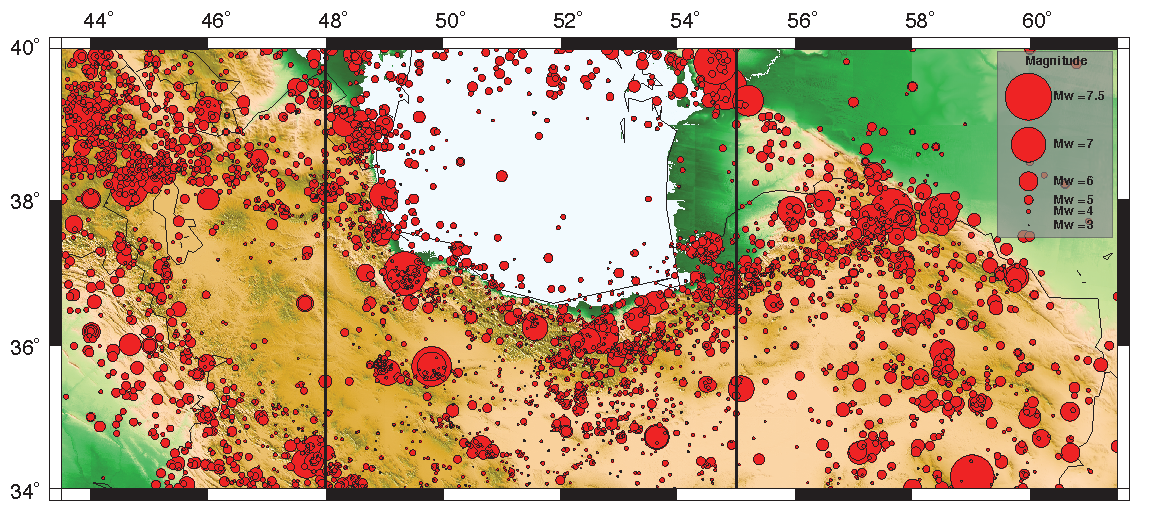
\includegraphics[scale=0.8]{figures/pdf/Figure3.pdf} 
\caption{Declustered instrumental seismicity map (after 1900) of Northern Iran. The study areas are separated at longitude of 48$^{\circ}$ and 55$^{\circ}$ . } 
\label{fig:instrumental}
\end{figure}





\section{Completeness tests}
For the smoothed seismicity method, completeness of each magnitude in the catalog is an important factor. To access catalog completeness, according to \citet{Frankel1995}, we made plots of the cumulative number of events against time for different regions.   Fig.~\ref{fig:comptest} shows the completeness of data for each magnitude threshold in three different regions.
A uniform rise of cumulative number of earthquake in each magnitude big, defines the threshold for catalog completeness.

\begin{figure} [H]
\centering
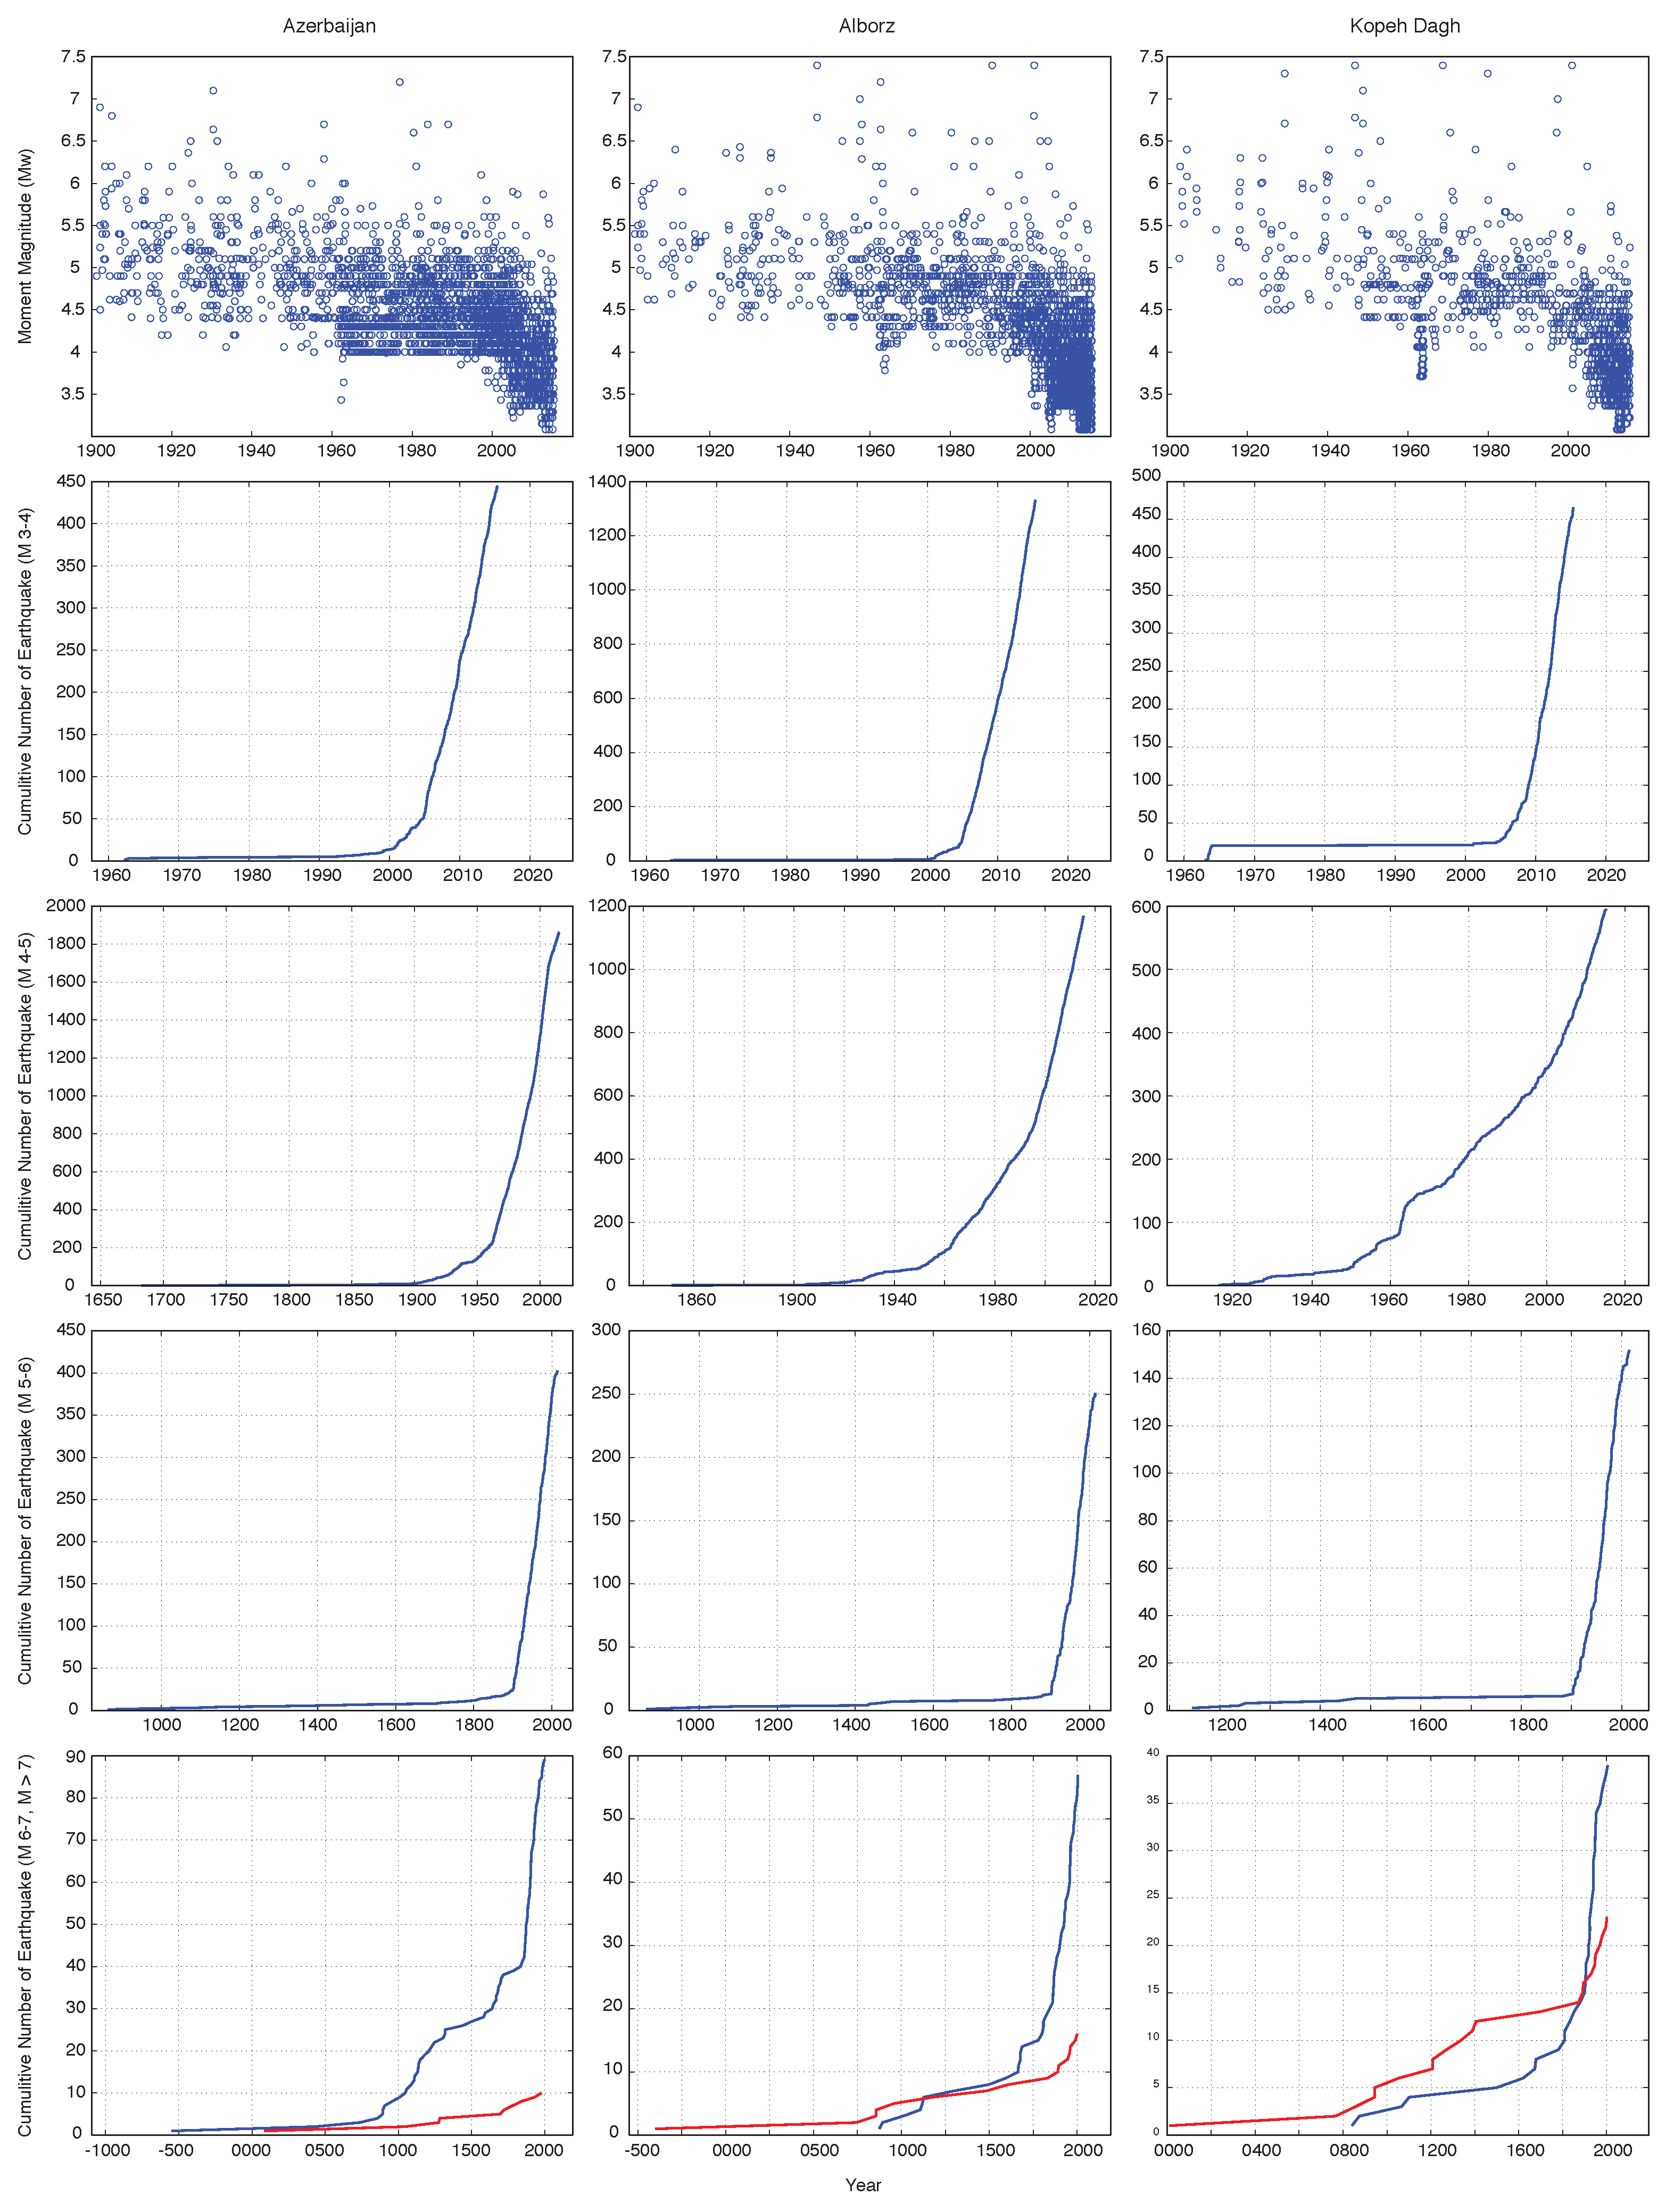
\includegraphics[scale=0.3]{figures/pdf/Figure4.pdf} 
\caption{Completeness test for earthquakes occurred in the three study regions. Red lines represent $M_w > 7$ }
\label{fig:comptest}
\end{figure}

We assume the catalog for earthquakes with magnitude greater than $M_w=7$ is complete from the first historical earthquake report. Table 1 presents the completeness of catalog of each region for different moment magnitudes.

\begin{table}[h]
\centering
\caption{Completeness threshold of three tectonic seismic regions.}
\begin{tabular}{cccc}
 ~           & Azerbaijan & Alborz & Kopeh Dagh \\ \hline
3-4         & 2004       & 2004   & 2005       \\ \hline
4-5         & 1960       & 1960   & 1960       \\ \hline
5-6         & 1900       & 1900   & 1900       \\ \hline
6-7         & 1844       & 1809   & 1810         \\ \hline
7 $< $    &  85          & -400    & 10         \\ \hline
\end{tabular}
\end{table}


\section{ Gutenberg-Richter Parameters}
For each of the three seismic regions, Gutenberg-Richter parameters and Max magnitude ($M_{max}$) were calculated using Seismic Hazard Assessment code (HA3) \citep{kijko2004}. The regional maximum magnitude for each region is estimated by the \citet{Kijko1989} method, which is implemented in the HA3 package. For smoothed seismicity areas, $b-value$ is assumed constant. The $a-value$ can vary spatially and is determined by counting earthquakes above $M$ 3.0 in grid cells.\\
\noindent
\citet{Karimiparidari2013} applied the Maximum Curvature (MAXC) technique \citep{Wyss1999, Wiemer2000} by ZMap \citep{Wiemer2001} to calculate the level of completeness of instrumental part of the catalog. In this study we use those magnitudes of completeness as the magnitude threshold in the calculation of the seismicity parameters. We also used the seismicity parameters of this study \citep{Karimiparidari2013} as the priory information in HA3 code. The updated values are displayed in Table 2. \\
\noindent
Following the \citet{Karimiparidari2013}, we assume the catalog is complete for earthquakes with magnitude 4.5, 4.4, and 4.5 for Azerbaijan, Alborz and Kopeh-Dagh tectonic seismic regions, respectively. The completeness of each region can be seen easily from the scatter plot of completeness test. 

\begin{table}[h]
\centering
\caption{Seismicity parameters for three tectonic seismic regions.}
    \begin{tabular}{ccccc}
    ~                   & $b-value$            & $\lambda$                  & $M_{max}$ Calculated & $M_{max}$ obseved \\ \hline
    Azerbaijan    & 1.06 $\pm$ 0.03  & (1.827  $\pm$ 0.216) & 7.78  $\pm$ 0.26           & 7.7          \\ \hline
    Alborz           & 1.1  $\pm$ 0.03   & (2.290  $\pm$ 0.282) & 7.91  $\pm$ 0.27           & 7.7          \\ \hline
    Kopeh Dagh & 0.97  $\pm$ 0.04 & (1.716  $\pm$ 0.243) & 7.67  $\pm$ 0.26           & 7.6          \\
    \end{tabular}
  
\end{table}



\section{Methodology for Hazard calculation}

To calculate the seismic hazard, we use spatially smoothed seismic hazard analysis \citep{Frankel1995}. In this model, seismic events are spatially gridded to cells. We are attempting to assess the relative likelihood of moderate earthquakes ($M_w > 4.5$), which cause structural damage. According to \citet{Frankel1995}, moderate earthquakes generally occur in areas that there have been significant numbers of events of magnitude 3 and above. Therefore, these events provide a reasonable guide to where moderate earthquakes will most likely occur. Since the catalog's completeness for $M3+$ and $M4+$ is different, we use two magnitude completeness range for less than $M_w5$ . Category of 5+ and others (M6+ and M7+) assume that future $M_w4.5$ events will occur near where they have occurred in the past. \\
\noindent
According to \citep{BHRC2014}, $M_w5$ is considered as a threshold magnitude to structural damage. In the smoothed seismicity method, the model uses each event location as a point source, hence $M_w4.5$ could be damaging earthquake if it occurs very close to the structure. In this study, in order to consider the probabilistic seismic hazard of both models, we defined two models based on $M_w5$ and $M_w4.5$ as a threshold magnitude for seismic hazard calculation with weight of 0.7 and 0.3, respectively.\\
\noindent
According to \citet{Frankel1995}, we count the number of earthquake $n_i$ with magnitude above $M{_R{_e{_f}}}$ in each cell of a grid with spacing of $0.1^{\circ}$ in both latitude and longitude (about 11 km). This count shows the maximum likelihood estimate of $10^a$ for that mentioned cell \citep{Weichert1980, Bender1983} for earthquakes with magnitude greater than $M{_R{_e{_f}}}$. Applying the Herrmann formula \citep{Herrmann1977}, the values of $n_i$ are converted from cumulative values (number of events above $M{_R{_e{_f}}}$) to incremental values (number of events from $M{_R{_e{_f}}}$ to $M{_R{_e{_f}}} +\Delta M$ ). The grid of $n_i$ values is spatially smoothed by multiplying by a Gaussian function with correlation distance c. For each cell $i$, the smoothed value $\tilde{n}_i$ is obtained from \citet{Frankel1995}


\begin{equation}
\tilde{n_i}=\frac{\sum_{j} n_{j} e^{\frac{-\Delta_{ij}^{2}}{c^2}}}{\sum_{j} e^{\frac{-\Delta_{ij}^{2}}{c^2}}},
\end{equation}

\noindent
where,  $\tilde{n}_i$  is normalized to preserve the total number of events. $\Delta{_i{_j}}$ is the distance between the $i{_t{_h}}$ and $j{_t{_h}}$ cell. The sum is calculated over cells $j$ within a distance of $3c$ of cell $i$.\\
\noindent
For a grid of sites and by using $\tilde{n}_i$ from Eq. (1), the annual probability of exceeding specified ground motions is calculated. For each site, the values of $\tilde{n}_i$ are binned by their distance from that site, in a way that $N_k$ denotes the total of $\tilde{n}_i$ values for cells within a certain distance increment of the site. Now the annual rate $\lambda (u> u_0 )$ of exceeding ground motion $u_0$ at a specific site is determined from a sum over distance and magnitude \citet{Frankel1995}:



\begin{equation}
\lambda(u>u_{0}) = \sum_{k}\sum_{l}10^{[log(\frac{N_{k}}{T}-b(M_l-M{_r{_e{_f}}}))]} p(u>u_0 | D_k ,M_l),
\end{equation}

\noindent
where $k$ is the index for the distance bin, and $l$ is the index for the magnitude bin; $T$ is the time in years of the earthquake catalog used to determine $N_k$. Annual rate of earthquakes in the distance bin $k$ and magnitude bin $l$ is the first factor in the summation. The $b-value$ is considered uniform throughout most of the area. $P(u>u_0 | D_k,M_l )$ is the probability that for an earthquake at distance $D_k$ with magnitude $M_l$, u at the site will exceed  ground motion $u_0$. This probability depends on the attenuation relation and the standard deviation (aleatory variability) of the ground motion for any specific distance and magnitude \citep{Frankel1995}



\section{Attenuation relationship}
The choice of a ground motion attenuation model is of great importance since attenuation has proven to be a highly influential factor of seismic hazard. \citet{Zafarani2014} used 163 free-field acceleration time histories recorded at epicentral distance of up to 200 km from 32 earthquakes to investigate the predictive capabilities of the local, regional, and next generation attenuation (NGA) ground-motion prediction equations and determined their applicability for northern Iran. After evaluating different Ground Motion Prediction Equations, \citet{Kalkan2004}, \citet{Chiou2008}, and \citet{Boore2008} represented suitable performance for  PGA  with LLH (Log-Likelihood method) score of 1.54, 1.55, and 1.59. Mean of the mentioned attenuation relationships (not shown here), are very close together, especially at higher magnitude. Using \citet{Scherbaum2009} approach and \citet{Zafarani2014} coefficients we calculated the logic tree weights as 0.3376, 0.3354, and 0.3270, respectively. Getting close mean values and logic tree weights, in order to consider the epistemic uncertainty, instead of using several GMPEs we use the top rank GMPE (i.e.  \citet{Kalkan2004} ) with  $\pm$ standard deviation with weight of 0.2 (for each of standard deviation branches) and 0.6 for the mean value.    \\

\noindent

The attenuation relationship is:

\begin{equation}
ln\ (Y) = b_1 + b_2(M_w-6) + b_3( M_w-6)^{2}+ b_5ln\ r + b_V \ ln(V_S/V_A) \  with \  r= \sqrt{R{r^2_{cl} + h^2}}  
\end{equation}

where $Y$ is in $g$, $b_1 = 0.393$, $b_2 = 0.576$, $b_3 = -0.107$, $b_5 = -0.899$, $b_V = -0.200$, $V_A = 1112$, $h(km) = 6.91$, $\sigma_{ln\ Y} = 0.612$.




\section{Hazard Calculation}

The PGA hazard maps have been computed for a 10\% and 2\% exceedance probability in 50 years, corresponding to a return period of 475 and 2475 years, from gridded values of historical and instrumental seismic activity. These levels of exceedance are a standard practice in seismic designs \citep{BHRC2014}.\\
\noindent
Even though in this study we are interested in investigating seismic hazard study in the northern Iran, in the smoothed seismicity method we defined the border of the study region broadly enough to ensure that the seismicity outside of the border doesn't affect the study area.  In addition, the border of the influenced area should surround the area of interest as uniformly as possible \citep{Lapajne1997}. Therefore, our study region includes parts of central and eastern Iran and the Zagros tectonic seismic regions.\\
\noindent
We calculated the $a-values$ for each cell and spatially smoothed over a grid of $0.1 \times 0.1$ in latitude and longitude. We assume magnitude increment as $\Delta_M = 0.1$. In this model, events are not assigned to specific faults and are assumed to be potential seismogenic sources, and are spatially gridded to cells. \\
\noindent
Different correlation distances have been used in different studies, which are generally dependent on the accuracy of the location of the recorded earthquakes. \citet{Frankel1995} and \citet{Boyd2008} assumed the correlation distance to be 50 $km$. \citet{Barani2007} used distance of 25 $km$ based on previous studies that suggested the correlation function of the Alps and Apennines in Italy. \citet{Foteva2006} used 10 and 15 km in a different model. Correlation distance is a very sensitive parameter in smoothed seismic hazard maps, and it is a factor of uncertainty in earthquake location. In the Iranian earthquake catalog, the magnitude uncertainties were assumed to be in the interval of $\pm$ 0.25 magnitude units and epicentral errors of $\pm$ 30 km \citep{Zare2012}. Even though these error margins are different for different events in terms of instrumental or historical events, in this study we assumed the correlation distance as 30 km because of the lack of knowledge about other historical events. Regarding the study domain and the 0.1 grid size, the total number of source is grid sites is 11651. Even though \citet{Kalkan2004} derived the attenuation relationship up to 250 km, since \citet{Zafarani2014} used data up to 200 km to evaluate the GMPEs, we set the model to compute the ground motions at distances of less than 200 km.
Fig.~\ref{fig:10percent} and Fig.~\ref{fig:2percent} show the seismic hazard map based on background seismicity for 10\% and 2\% probability of exceedance in 50 years, respectively. The areas of large probabilistic ground motions clearly coincide with zones with a large number of events with magnitude 3 and larger.


\begin{figure} [H]
\centering
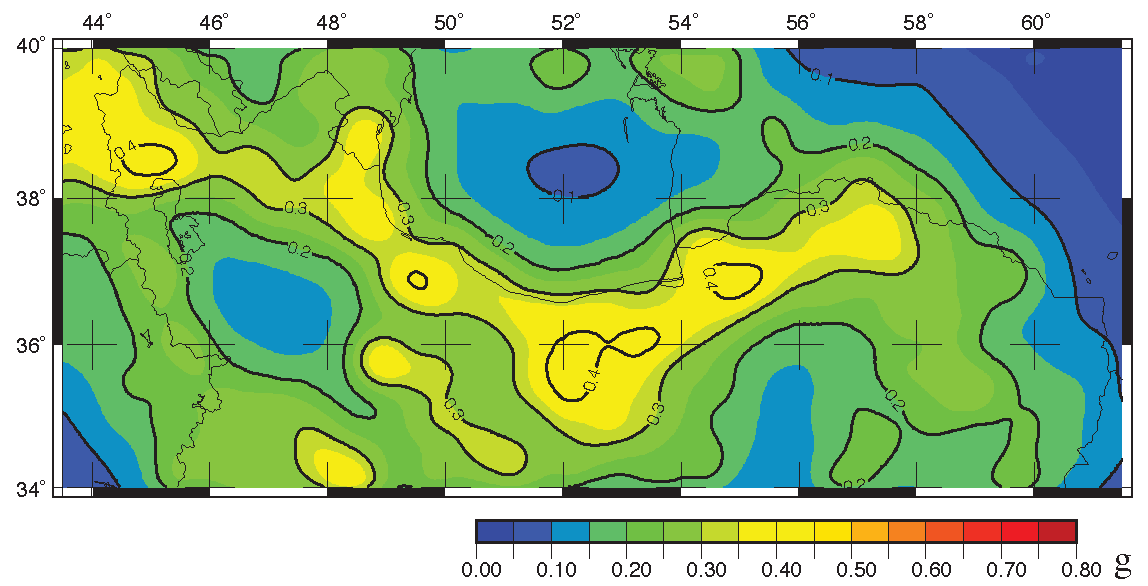
\includegraphics[scale=0.8]{figures/pdf/Figure5.pdf} 
\caption{Probabilistic PGA (10\% in 50 years), based on smoothed seismicity for Northern Iran }
\label{fig:10percent}
\end{figure}



\begin{figure} [H]
\centering
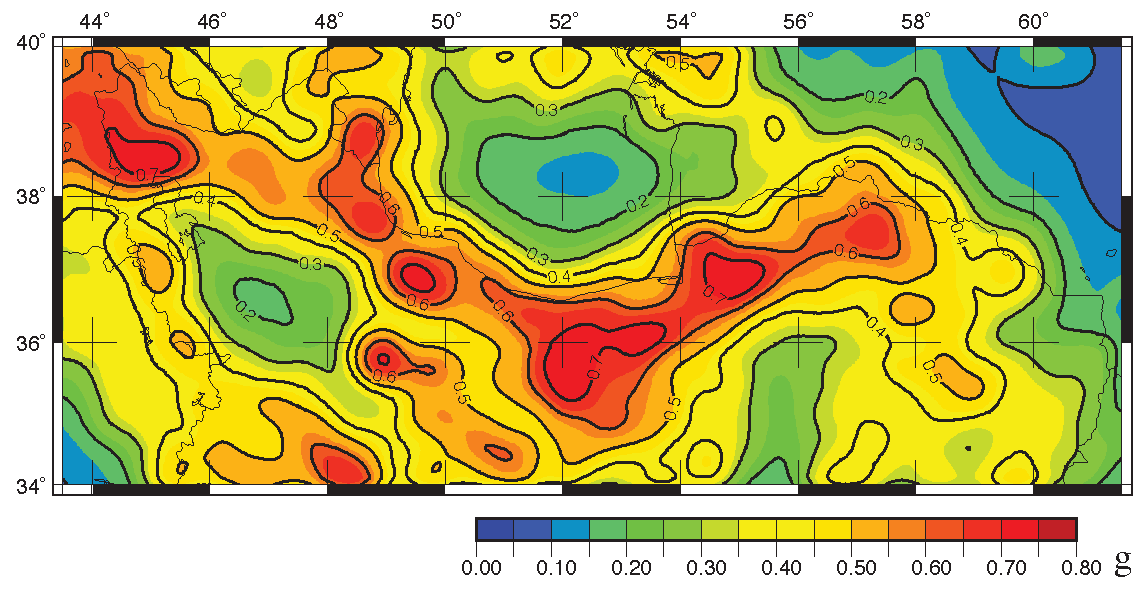
\includegraphics[scale=0.8]{figures/pdf/Figure6.pdf} 
\caption{Probabilistic PGA (2\% in 50 years), based on smoothed seismicity for Northern Iran}
\label{fig:2percent}
\end{figure}






\section{Discussion}

Seismic hazard in northern Iran is computed based on background seismicity and projected on a set of hazard maps. The results obtained are represented as maps for the spatial distribution of horizontal peak ground acceleration with 10\% and 2\% probability of exceedance in 50 years, which correspond to the return period of 475 and 2475 years. The areas of large probabilistic ground motions clearly coincide with zones with a large number of events of magnitude 3.0 and larger. Figure 5 presents the map of PGA for 10\% exceedance in 50 years. The highest and the lowest contour values are 0.44g and 0.12g, respectively. The highest and lowest values in Fig.~\ref{fig:10percent} are 0.74g and 0.19g, respectively. (We disregarded the values in the Caspian Sea and also close to the study region's borders). Highest hazards are established in the Alborz tectonic seismic region in the city of Damavand, about 55 km east of Tehran city in Tehran province. Lowest hazards are established in the Azerbaijan tectonic seismic province, about 31 km east of Shahin Dezh in West Azerbaijan province. Also many other places are in higher hazard zone both in Azerbaijan and and Alborz seismic tectonic regions (See Fig.~\ref{fig:10percent} and Fig.~\ref{fig:2percent}). Many seismic hazard analysis studies have been done in the region based on different methods. Table 3 presents the PGA value for some of the major cities in northern Iran from different studies.

\begin{table}[h]
\centering
\caption{Comparison of PGA, from different studies for selected cities in Northern Iran. (V2009:  \citet{vafaie2011}), G2008: \citet{Ghodrati2008}, G2010: \citet{Ghodrati2010},  Ah2013: \citet{Ahmadi2013}, G2003:  \citet{Ghodrati2003}, G2011: \citet{Ghodrati2011}, Ab2014: \citet{Abdollahzadeh2014} , Ra2012: \citet{Rahgozar2012}) }
\begin{tabular}{ | c | c | c | c | c | c | c | c | c | c |}


\hline

	
	\multirow{2}{*}{Cities} & \multirow{2}{*}{Lon} & \multirow{2}{*}{Lat} & \multicolumn{2}{|c|}{This study} & \multirow{2}{*}{2800} & Zare & \multicolumn{3}{|c|}{Other Refrences}    \\ 
	\cline{4-5}  \cline{8-10}  &  &  & 10\% & 2\% &  &  2012 & 10\% & 2\% & ref \\ \hline
	Orumyeh & 45.07 & 37.55 & 0.22 & 0.39 & 0.3 & 0.35-0.5 &  &  &  \\ \hline
	Tabriz      & 46.3     & 38.06 & 0.27& 0.50 & 0.35 & 0.35-0.5 & 0.2- 0.65 & 0.3 to 0.9 & V2009 \\ \hline
	Ardabil    & 48.28 & 38.25 & 0.36 & 0.63 & 0.3 & 0.35-0.5 &  &  &  \\ \hline
	Manjil     & 49.40 & 36.74 & 0.39 & 0.71 & 0.35 & 0.65 $<$ & 0.25 & 0.4 & G2008 \\ \hline
	Rasht     & 49.58 & 37.27 & 0.33 & 0.55 & 0.3 & 0.5-0.65 & 0.1 & 0.2 & G2008 \\ \hline 
	Arak       & 49.68 & 34.09 & 0.24 & 0.48 & 0.25 & 0.35-0.5 & 0.16-0.36 & 0.25-0.55 & G2010 \\ \hline
	Qazvin   & 50.00 & 36.26 & 0.27 & 0.50 & 0.35 & 0.35-0.5 & 0.31 & 0.42 & Ah2013 \\ \hline
	 \multirow{2}{*}{Tehran}  & \multirow{2}{*}{51.42} & \multirow{2}{*}{35.69} & \multirow{2}{*}{0.35} & \multirow{2}{*}{0.59} & \multirow{2}{*}{0.35} & \multirow{2}{*}{0.35-0.5} & 0.37-0.415 &  &  G2011 \\ 
	 \cline{8-10}	             &  &  &  &  &  &  & 0.27-0.46 & 0.35 & G2003\\ \hline
	Gorgan & 54.43 & 36.83 & 0.39 & 0.69 & 0.3 & 0.35-0.5 & 0.34 & 0.3$<$ & Ab2014\\ \hline
	Bojnurd & 57.33 & 37.47 & 0.38 & 0.68 & 0.3 & 0.35-0.5 &0.16-0.2  & 0.32-0.45  & Ra2012  \\ \hline
	Mashhad & 59.6 & 36.29 & 0.16 & 0.28 & 0.3 & 0.35-0.5 &  &  & Ak2011 \\ \hline

\end{tabular}

\end{table}


According to Table 3, the results of smoothed seismicity  are comparable with many other studies that considered faults and seismogenic zones. According to \citet{BHRC2014}, our results show that the smoothed seismicity approach gives reasonable regionalized results for 10\% probability of exceedance even when there is no need to introduce seismogenic zones. However, in regions for which the catalog is not complete or the study area is near the fault, probabilistic seismic hazard studies, which are implemented by seismic source, should be conducted. 



\section{Conclusion}

The aim of this study is to conduct a new probabilistic seismic hazard assessment for northern Iran using updated seismic catalogs. Seismic hazard is evaluated over three regions (Azerbaijan, Tehran, Kopeh-Dagh) using the smoothed background seismicity. According to our study, in the Alborz  and Azerbaijan regions substantial seismic hazard is observed.  We studied probabilistic seismic hazard based on smoothed seismicity using historical and instrumental data. The results of this paper can be addressed in three main conclusions. First, probabilistic seismic hazard analysis using smoothed seismicity is sufficient for 10\% probability of exceedance. Second, since this study is based solely on historical and instrumental data, places with very close PGA values to those studies with considering faults as a primary source of seismicity, show normal and predictable seismic activity. Third, places with lower hazard values compared to other studies show anomalous seismic activity and suggest the idea of expecting more and bigger events in the future. As mentioned before, probabilistic seismic hazard analysis based on smoothed seismicity is very sensitive to input parameters (e.g., correlation distance, $b-value$, catalog completeness, and threshold magnitude for structural damage). Studying the sensitivity rate of these parameters could develop a more trustworthy result. Maps presented in this paper are for illustrative purposes only, and are not intended to be used in any application. 



\section{Acknowledgements}

 We express our appreciation to Art Frankel, PhD, of the U.S. Geological Survey, Washington, DC, who kindly provided the Smoothed Probabilistic Seismic Hazard Analysis (PSHA) package. We are also very thankful to Andrzej Kijko, PhD, Director of the University of Pretoria Natural Hazard Centre, Pretoria, Africa, who generously provided the software to compute seismicity parameters. We wish to thank Mehdi Zare, PhD, engineering seismologist and Associate Professor of Engineering Seismology at the International Institute of Earthquake Engineering and Seismology, Tehran, Iran, for  kindly providing the uniform historical seismic catalog. We also are very grateful to the International Institute of Earthquake Engineering and Seismology of Iran, Tehran, Iran, for providing the uniform instrumental earthquake catalog. 





\newpage

%\section*{References}

{
\renewcommand{\bibname}{}
\bibliographystyle{ascelike}
\bibliography{PSHA}
}



\end{document}

